
\section{Own implementation: lid-driven cavity}

In our own implementation \cite{source} a lid-driven cavity in 3D with D3Q19 model was implemented. The streaming and collision were implemented as described before in two different steps. Further figures are received on the 5000th iteration. The initial velocity of the lid was 0.01 and the size of the cavity was 50 cells. On Figure \ref{fig:density-paraview} a density distribution is shown. In both corners of the cavity can be observed high and low density zones, which response to high and low pressure respectively. This behaviour is correct for lid-driven cavity systems. 

The resulted velocity stream field can be seen on Figure \ref{fig:stream-field-paraview}. There is a vertex in the left lower corner, which response to the stream with the direction (anticlockwise) other than the direction (clockwise) of the main(big) vertex. The result of the LBM simulation responses to the result of the lid-driven cavity simulation with Navier-Stokes method.

\begin{figure}[H]
  \centering
  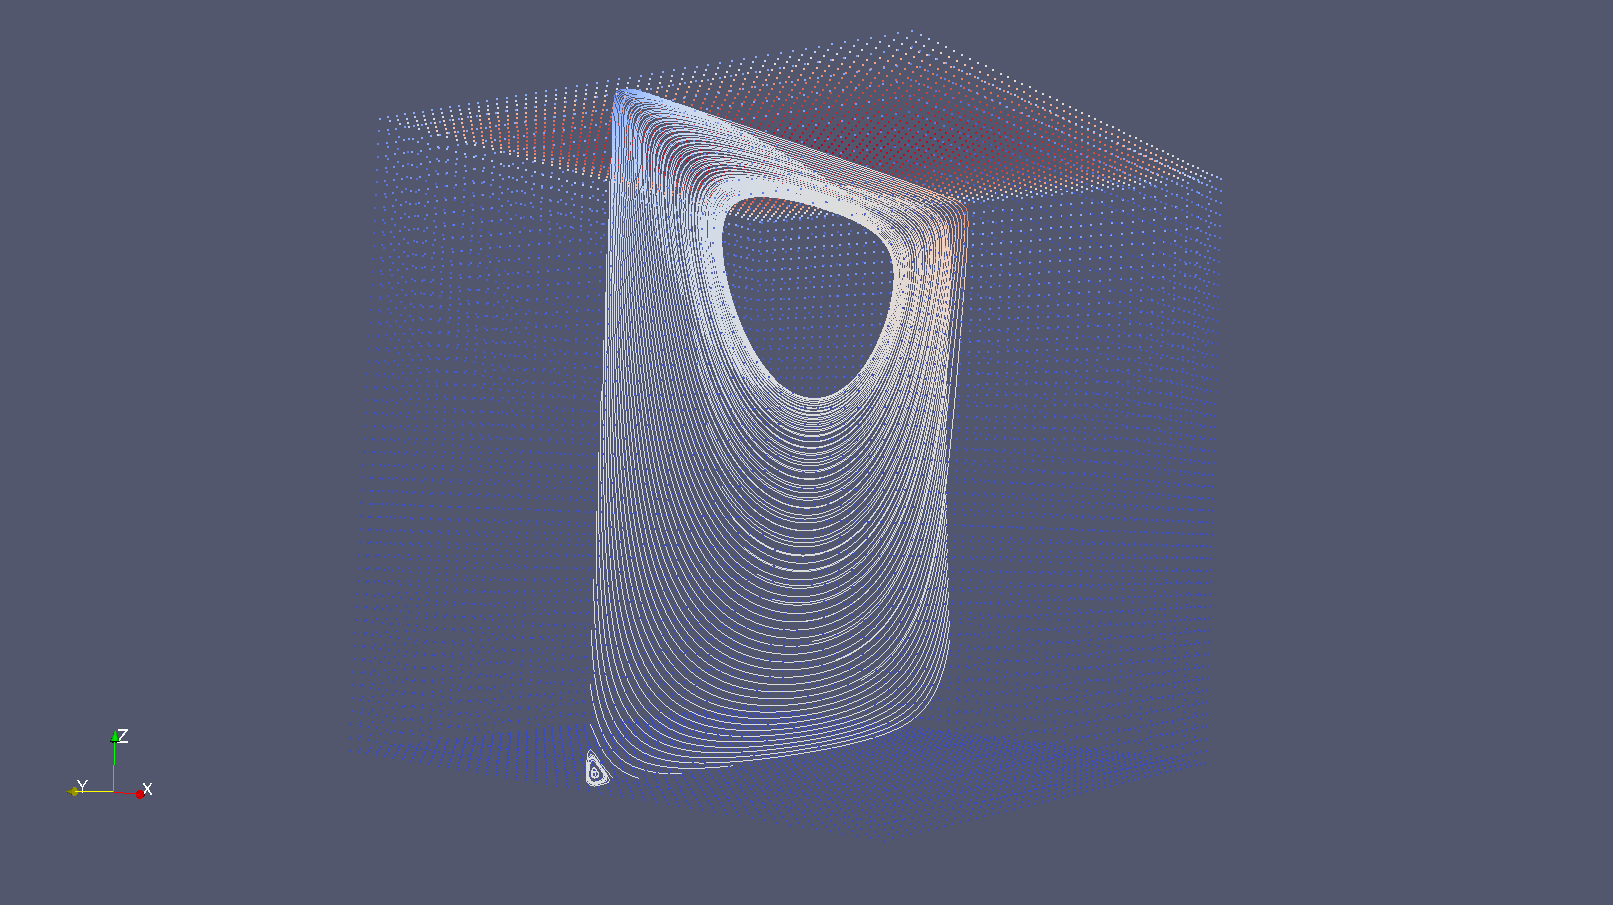
\includegraphics[width=0.7\textwidth]{img/fig10.png}
  \caption{Visualization of density of the lid-driven cavity simulation with D3Q19 model.}\label{fig:density-paraview}
\end{figure}

\begin{figure}[H]
  \centering
  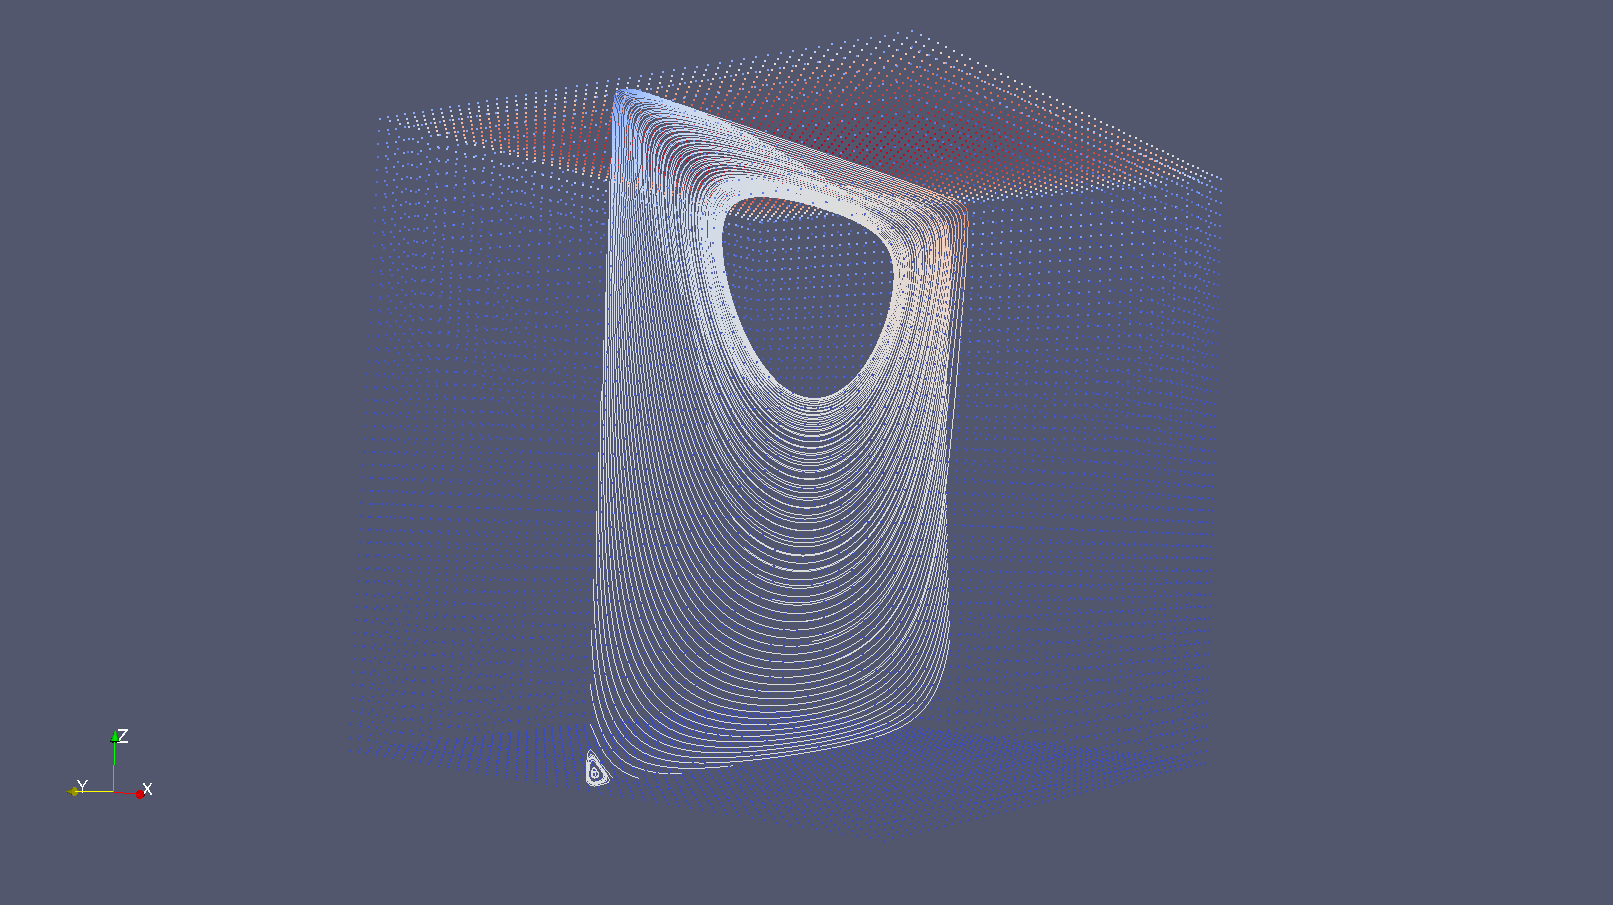
\includegraphics[width=0.6\textwidth]{img/fig11.png}
  \caption{Visualization of the velocity stream field in the lid-driven cavity simulation with D3Q19 model.}\label{fig:stream-field-paraview}
\end{figure}